\chapterimage{images/activities.jpg} % Chapter heading image


\chapter{Activities and Their Lifecycles}
An activity is a single, focused thing that the user can do.
Almost all activities interact with the user, so the Activity class takes care of creating a window for you in which you can place your UI with \texttt{setContentView(View)}. \todo{check if still applicable}
Unlike programming paradigms in which apps are launched with a main() method, the Android system initiates code in an Activity instance by invoking specific callback methods that correspond to specific stages of its lifecycle.

\begin{framed}
	\todo{Aanpassen}
	This chapter has an example application which you can find here \cite{GoogleDevelopers2018}.
	The link contains the steps which youy need to take to build the application.
	The final code can be found on \url{https://github.com/eothein/ActivityProject}	
\end{framed}


\section{Activities}
The Activity class serves as the entry point for an app’s interaction with the user, providing the window in which the app draws its UI.
This window typically fills the screen, but may be smaller than the screen and float on top of other windows.
You implement an activity as a subclass of the Activity class.
Generally, one activity implements one screen in an app.
For instance, one of an app’s activities may implement the Preferences screen, while another activity implements the Compose Email screen.

Most apps contain multiple screens, which means they comprise multiple activities.
Typically, one activity in an app is specified as the main activity, which is the first screen to appear when the user launches the app.
Each activity can then start another one in order to perform different actions.
For example, the main activity in a simple e-mail app may provide the screen that shows an e-mail inbox.
From there, the main activity might launch other activities that provide screens for tasks like writing e-mails and opening individual e-mails.

Although activities work together to form a cohesive user experience in an app, each activity is only loosely bound to the other activities.
It is good practice to keep dependencies between activities to a minimum.
Sometimes activities start up activities belonging to other apps.
For example, a browser app might launch the Share activity of a social-media app.

To use activities in your app, you must register information about them in the app’s manifest, and you must manage activity lifecycles appropriately.

\subsection{One Activity to rule them all}
In the past Android recommended to use one Activity for a single, focuses task for your application.
This resulted in applications with many Activities, all serving a certain purposes.
This architecture had several drawbacks:

\begin{enumerate}
	\item Toolbar configuration and views are handles on different places
	\item You had to rely on the Android Framework to change content
	\item Previous Activities with views could still exist in the stack, which can cause an out-of-memory exception in endless navigation applications
	\item Side menu implementation was difficult.
\end{enumerate}

Android is introducing the Navigation component as a framework for structuring your in-app UI, with a focus on making a single-Activity app the preferred architecture.
Although we are not going to cover the Navigation Component (still in $\alpha$ phase), later in this book we will use the single activity architecture with the corresponding features.
For this chapter however, we will use multiple activities for educational purposes.

\section{The Activity Lifecycle}
As stated before, an activity is a single, focused thing that the user can do.
Almost all activities interact with the user, so the Activity class takes care of creating a window for the UI.

Activities in the system are managed as an activity stack.
When a new activity is started, it is placed on the top of the stack and becomes the running activity.
The previous activity always remains below it in the stack, and will not come to the foreground again until the new activity exits.

The activity lifecycle is demonstrated in figure \ref{fig:lifeCycle1}, which shows the different states and transitions an activity is able to make.
The same model, but maybe a but more easy to read is shown in figure \ref{fig:lifeCycle2}.
It is up to the reader to see that these figures illustrate the same concept.

As Activities are created and destroyed, they move in and out of the stack \footnote{Activities in the system are managed as an activity stack.
When a new activity is started, it is placed on the top of the stack and becomes the running activity -- the previous activity always remains below it in the stack, and will not come to the foreground again until the new activity exits.} (the "back stack").
As they do so, they transition through four possible states.

\begin{enumerate}
	\item \textbf{Active} - When an Activity is at the top of the stack it is the visible, focused, foreground Activity that is receiving user input.
		Android will attempt to keep it alive at all costs, killing Activities further down the stack as needed, to ensure that it has the resources it needs.
		When another Activity becomes active, this one will be paused.
	\item \textbf{Paused} - In some cases your Activity will be visible but will not have focus; at this point it’s paused.
		This state is reached if a transparent or non-full-screen Activity is active in front.
	\item \textbf{Stopped} - When an Activity isn’t visible, it “stops.” 
		The Activity will remain in memory; however, it is now a candidate for termination when the system requires memory elsewhere.
		When an Activity is in a stopped state, it is important to save data and the current UI state, and to stop any non-critical operations.
	\item \textbf{Inactive} - After an Activity has been killed, and before it’s been launched, it’s inactive.
		Inactive Activities have been removed from the Activity stack and need to be restarted before they can be displayed and used.
\end{enumerate}

\begin{figure}
	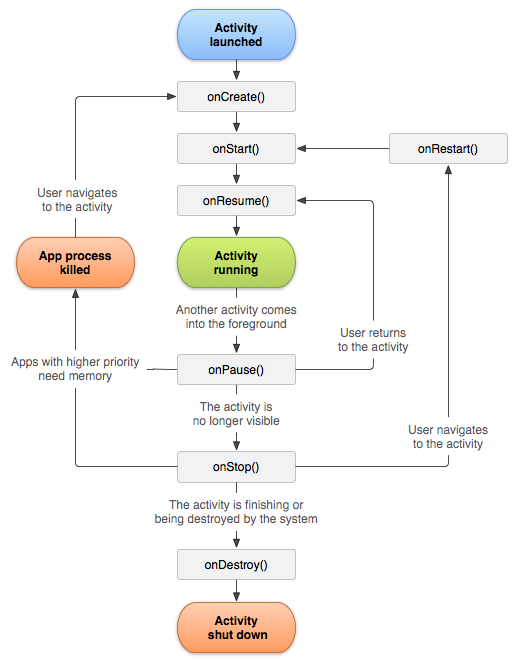
\includegraphics[width=\textwidth]{images/activity/activity_lifecycle1.png}
	\caption{The activity lifecycle, retrieved from \cite{Developers19}}
	\label{fig:lifeCycle1}
\end{figure}

\begin{figure}
	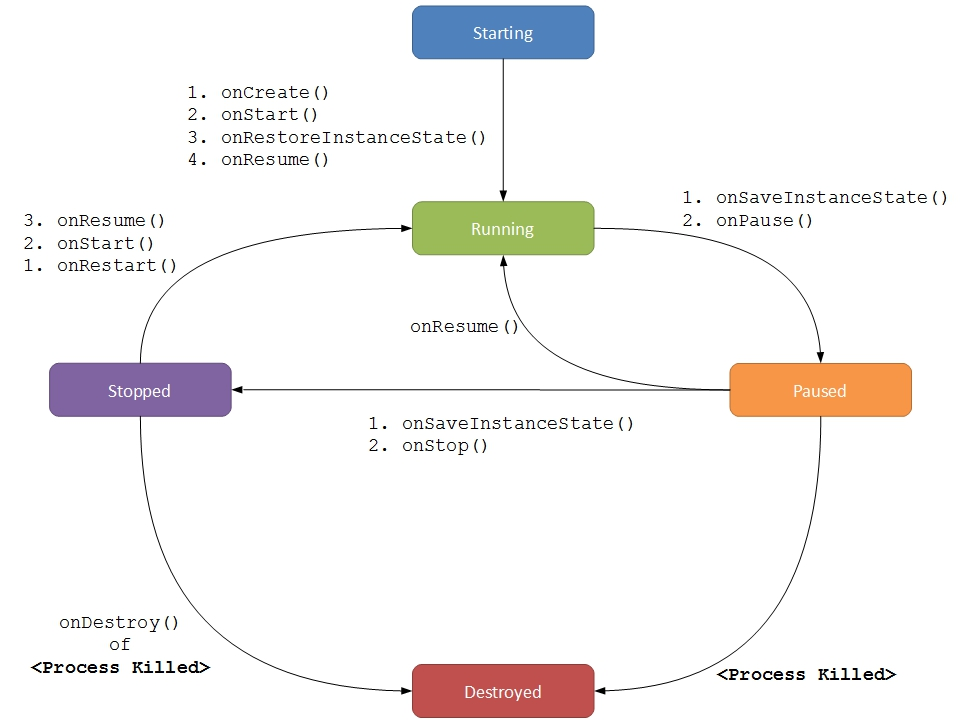
\includegraphics[width=\textwidth]{images/activity/activitylifecycle2.jpg}
		\caption{An even more simplified illustration of the activity lifecycle}
	\label{fig:lifeCycle2}
\end{figure}

For more information regarding the different life cylce callback, we refer the reader to \cite{Developers19}.

\subsection{Saving and restoring the state}
There are a few scenarios in which your activity is destroyed due to normal app behavior, such as when the user presses the Back button or your activity signals its own destruction by calling the finish() method.
The system may also destroy the process containing your activity to recover memory if the activity is in the Stopped state and hasn't been used for a long time, or if the foreground activity requires more resources.

When your activity is destroyed because the user presses  ``Back'' or the activity finishes itself, the system's concept of that Activity instance is gone forever because the behavior indicates the activity is no longer needed.
However, if the system destroys the activity due to system constraints (rather than normal app behavior), then although the actual Activity instance is gone, the system remembers that it existed.
When the user navigates back to it, the system creates a new instance of the activity using a set of saved data that describes the state of the activity when it was destroyed.
The saved data that the system uses to restore the previous state is called the \textbf{instance state} and is a collection of key-value pairs stored in a Bundle object.

By default, the system uses the Bundle instance state to save information about each View object in your activity layout (such as the text value entered into an EditText widget).
So, if your activity instance is destroyed and recreated, the state of the layout is restored to its previous state with no code required by you.
However, your activity might have more state information that you'd like to restore, such as member variables that track the user's progress in the activity.

\begin{exercise}
	Start the example application found in \url{https://github.com/eothein/ActivityProject}.
	Remove the id of the editText (\texttt{android:id="@+id/nameEditText"}).
	Fill in your name and turn the device.
	What do you see? What happens when you close the app or press the back button?
\end{exercise}

\subsubsection{Reacting to configuration changes}
Some device configurations can change during runtime (such as screen orientation, keyboard availability, and when the user enables multi-window mode).
When such a change occurs, Android restarts the running Activity ( onDestroy() is called, followed by onCreate()).
The restart behavior is designed to help your application adapt to new configurations by automatically reloading your application with alternative resources that match the new device configuration.

If restarting your activity requires that you recover large sets of data, reestablish a network connection, or perform other intensive operations, then a full restart due to a configuration change might be a slow user experience.
Also, it might not be possible for you to completely restore your activity state with the Bundle the system saves for you with the onSaveInstanceState() callback.
It is not designed to carry large objects (such as bitmaps) and the data within must be serialized and deserialized on the main thread, which can consume a lot of memory and slow down the configuration change.

\subsubsection{Persisting Data Between Launches}
As your activity begins to stop, the system calls the onStop() method so your activity can save state information using a collection of key-value pairs.
The default implementation of this method saves transient information about the state of the activity's view hierarchy, such as the text in an EditText widget or the scroll position of a ListView widget.

When your activity is recreated after it was previously destroyed, you can recover your saved state from the Bundle that the system passes to your activity.
Both the onCreate() and onRestoreInstanceState() callback methods receive the same Bundle that contains the instance state information.

Because the onCreate() method is called whether the system is creating a new instance of your activity or recreating a previous one, you must check whether the state Bundle is null before you attempt to read it.
If it is null, then the system is creating a new instance of the activity, instead of restoring a previous one that was destroyed.

Instead of restoring the state during onCreate() you may choose to implement onRestoreInstanceState(), which the system calls after the onStart() method.
The system calls onRestoreInstanceState() only if there is a saved state to restore, so you do not need to check whether the Bundle is null.

Caution: Always call the superclass implementation of onRestoreInstanceState() so the default implementation can restore the state of the view hierarchy.

Another way of tackling the problem is using Sharedpreferences, which is outlined in the following code example.

\lstinputlisting[firstline=28,lastline=66,language=Kotlin, caption={Persisting Data Between Launches with Shared Preferences}, label=code:KotlinSRPBook]{srccode/activities/MainActivity.kt}



\section{Starting a new activity}
An Intent encapsulates a request send to Android for some activity or other receiver to do something.
If the activity you intend to launch is one of your own, you may find it simplest to create an explicit Intent, naming the component you wish to launch.
For example, from within your activity, you could create an Intent like this:

\begin{lstlisting}
val intent = Intent(this, NextActivity::class.java)
// To pass any data to next activity
intent.putExtra("keyIdentifier", value)
// start your next activity
startActivity(intent)
\end{lstlisting}

This would stipulate that you wanted to launch the NextActivity.
NextActivity would need to have a corresponding <activity> element in your AndroidManifest.xml file.

\section{The Manifest File}
Each Android project includes a manifest file, AndroidManifest.xml, stored in the root of its project hierarchy.
The manifest defines the structure and metadata of your application, its components and its requirements.
In this section we will briefly describe what you can find in the manifest.
The next chapters will take a closer look at it.

\begin{itemize}
	\item It includes nodes for each of the Activities, Services, Content Providers, and Broadcast Receivers that make up your application and, using Intent Filters and Permissions, determines how they interact with each other and with other applications.
	\item The manifest can also specify application metadata (such as its icon, version number, or theme), and additional top-level nodes can specify any required permissions, unit tests, and define hardware, screen, or platform requirements.
	\item The manifest is made up of a root manifest tag with a package attribute set to the project’s package.
		It should also include an xmlns:android attribute that supplies several system attributes used within the file.
	\item Use the versionCode attribute to define the current application version as an integer that increases with each version iteration, and use the versionName attribute to specify a public version that will be displayed to users.
\end{itemize}

\section{Externalizing Resources}
It’s always good practice to keep non-code resources, such as images and string constants, external to your code.
Android supports the externalization of resources, ranging from simple values such as strings and colors to more complex resources such as images (Drawables), animations, themes, and menus.
Perhaps the most powerful externalizable resources are layouts.

By externalizing resources, you make them easier to maintain, update, optimize and manage.
This also lets you easily define alternative resource values for internationalization and to include different resources to support variations in hardware - particularly, screen size and resolution.

\subsection{Strings}
String resources are specified with the string tag and simple markup attributes can be added.
\subsection{Colors}
Use the color tag to define a new color resource.
Specify the color value using a \# symbol followed by the (optional) alpha channel, and then the red, green, and blue values.
\subsection{Drawables}
A drawable resource is a general concept for a graphic that can be drawn to the screen: bitmap and xml descriptions of graphics.
\subsection{Layouts}
Layout resources enable you to decouple your presentation layer from your business logic by designing UI layouts in XML rather than constructing them in code.
You can use layouts to define the UI for any visual component, including Activities, Fragments, and Widgets.
Once defined in XML, the layout must be “inflated” into the user interface.
Within an Activity this is done using setContentView (usually within the onCreate method), whereas Fragment Views are inflated using the inflate method from the Inflator object passed in to the Fragment’s onCreateView handler.
Using layouts to construct your screens in XML is best practice in Android.

\newpage
\section{Exercises}
In this lesson we will build our first working app, using activities, intents and some basic User Interface design.

\begin{exercise}
	In this exercise you create an Activity and count how many times each lifecycle method from the Activity will be called.
	In order to do this you should:
	\begin{enumerate}
		\item Create a new activity with all necessary triggers (all of them)
		\item Log each lifecycle method using a desired logging method.
			Look for some examples online to find the solution that suits you best.
		\item Use a counter variable for each lifecycle method which is incremented with each call of the lifecycle method.
			The user interface should be able to show this counter.
		\item Do this for the first activity.
	\end{enumerate}
	\label{ex:act1}
\end{exercise}

If you are unsure on how to create this functionality, I have one tip: Google!

\begin{exercise}
	Now it is time to create a second activity, with the same functionality as the former.
	We are going to allow the first Activity to start the second activity.
	When you close the second activity, you should see the first activity again.
	You should:
	\begin{enumerate}
		\item Add buttons to both activities (to start the second activity) and one to close the second activity
		\item Implement the method which starts the second activity when the button has been pressed.
		\item Implement the method which stops the second activity and returns to the first activity.
	\end{enumerate}
	\label{ex:act2}
\end{exercise}

At the moment the design of the application is not that important.
Just make sure that the above functionality is implemented.
Don't forget all the good coding standards you have learned during the past years.